\begin{figure}[htbp]

\begin{center}
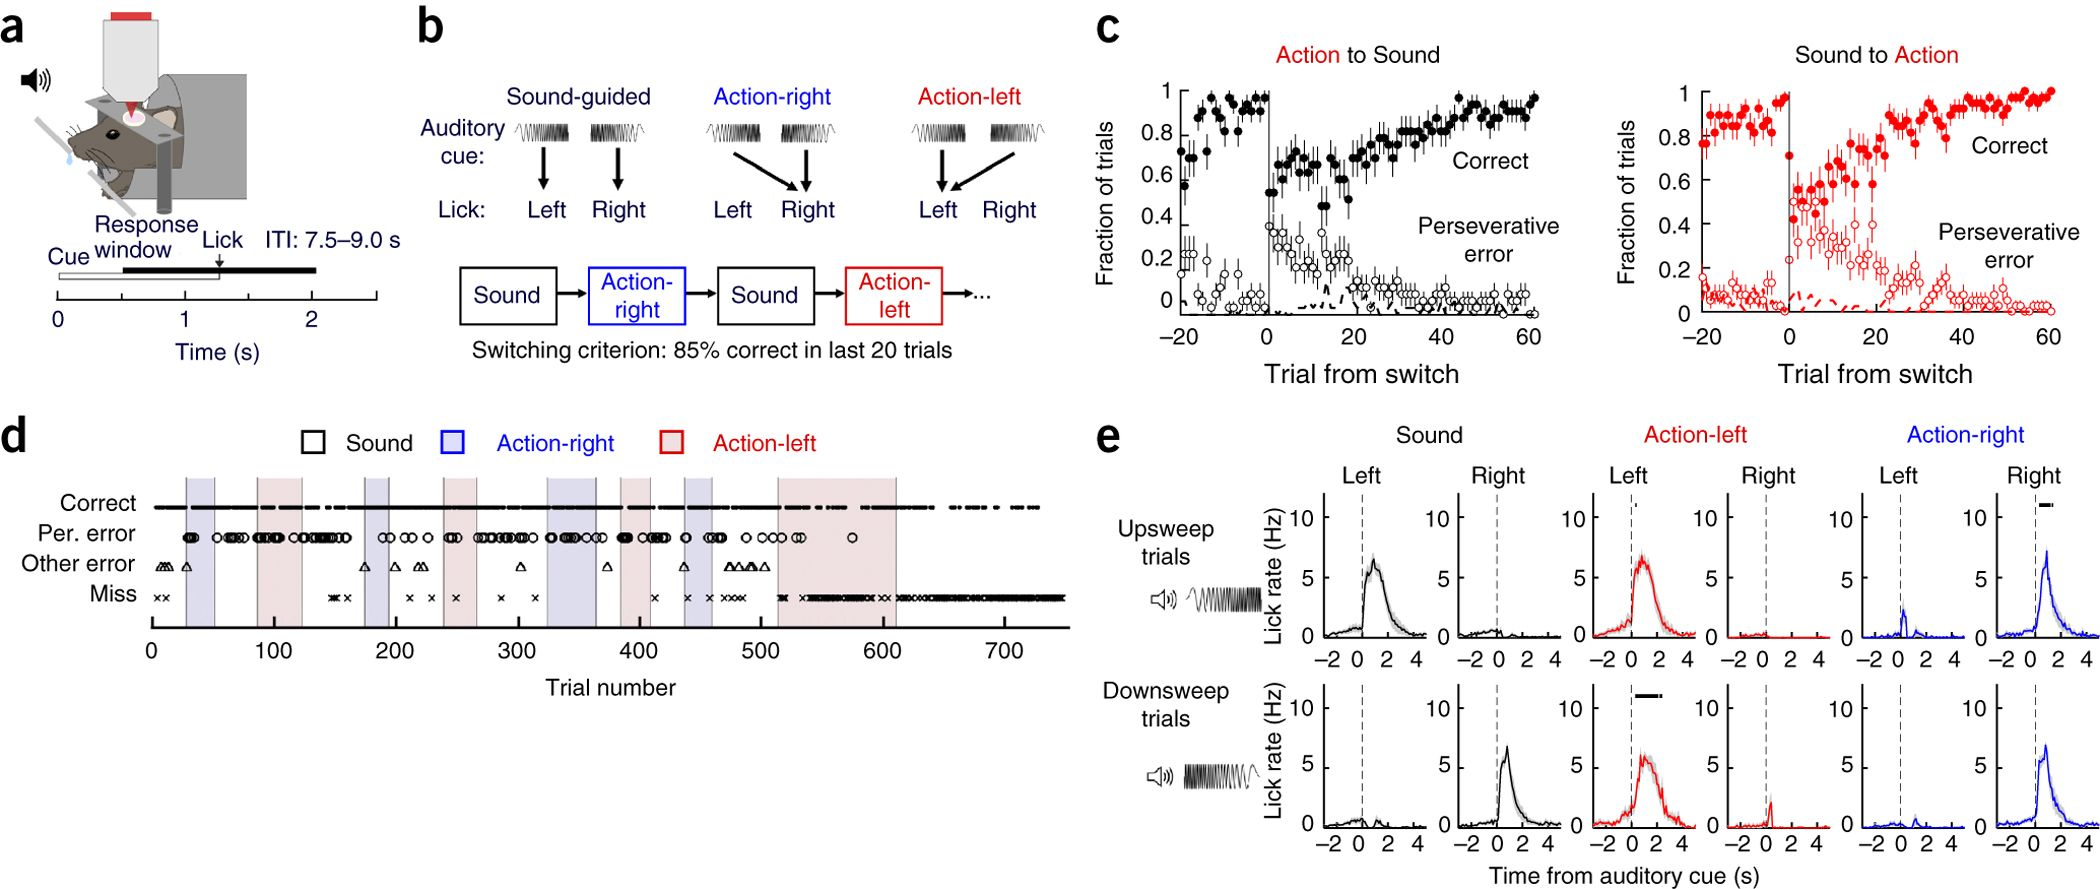
\includegraphics[width=\textwidth]{Figures/Chapter3/NN_fig1} 
\end{center}

\caption[Behavioral performance of head-fixed mice in an adaptive sensorimotor decision-making task]
{Behavioral performance of head-fixed mice in an adaptive sensorimotor decision-making task.
(a) Schematic of experiment. Each trial begins with an auditory cue. A response window starts 0.5 s after cue onset, during which the first lick is recorded as the response for that trial. Water reward is delivered contingent on a correct response. ITI, intertrial interval. (b) Schematic of stimulus–response mappings and block design. (c) Behavioral performance surrounding a block switch from action to sound (left) or sound to action (right). Filled circles, hit rate. Open circles, perseverative error rate. Dotted line, other error rate. $N=$ 33 action-to-sound switches and 38 sound-to-action switches. (d) Performance from one example behavioral session. Trial outcomes: correct (filled circles), perseverative error (open circles), other error (open triangles), or miss (cross). Vertical line, rule switch. (e) Left and right lick rates for upsweep or downsweep sound cues during all correct sound-guided (black), action-left (red) and action-right (blue) trials. For each choice direction, lick rates during action trials were compared to sound trials in 0.1 s bins; black bars, significant differences ($p<0.01$, paired t-test). All data presented as the $\mathit{mean}\pm\mathit{SEM}$. $N = 9$ sessions from 5 mice.}

\label{fig:NN_fig1}
\end{figure}

% \begin{FPfigure}

% \begin{center}
% 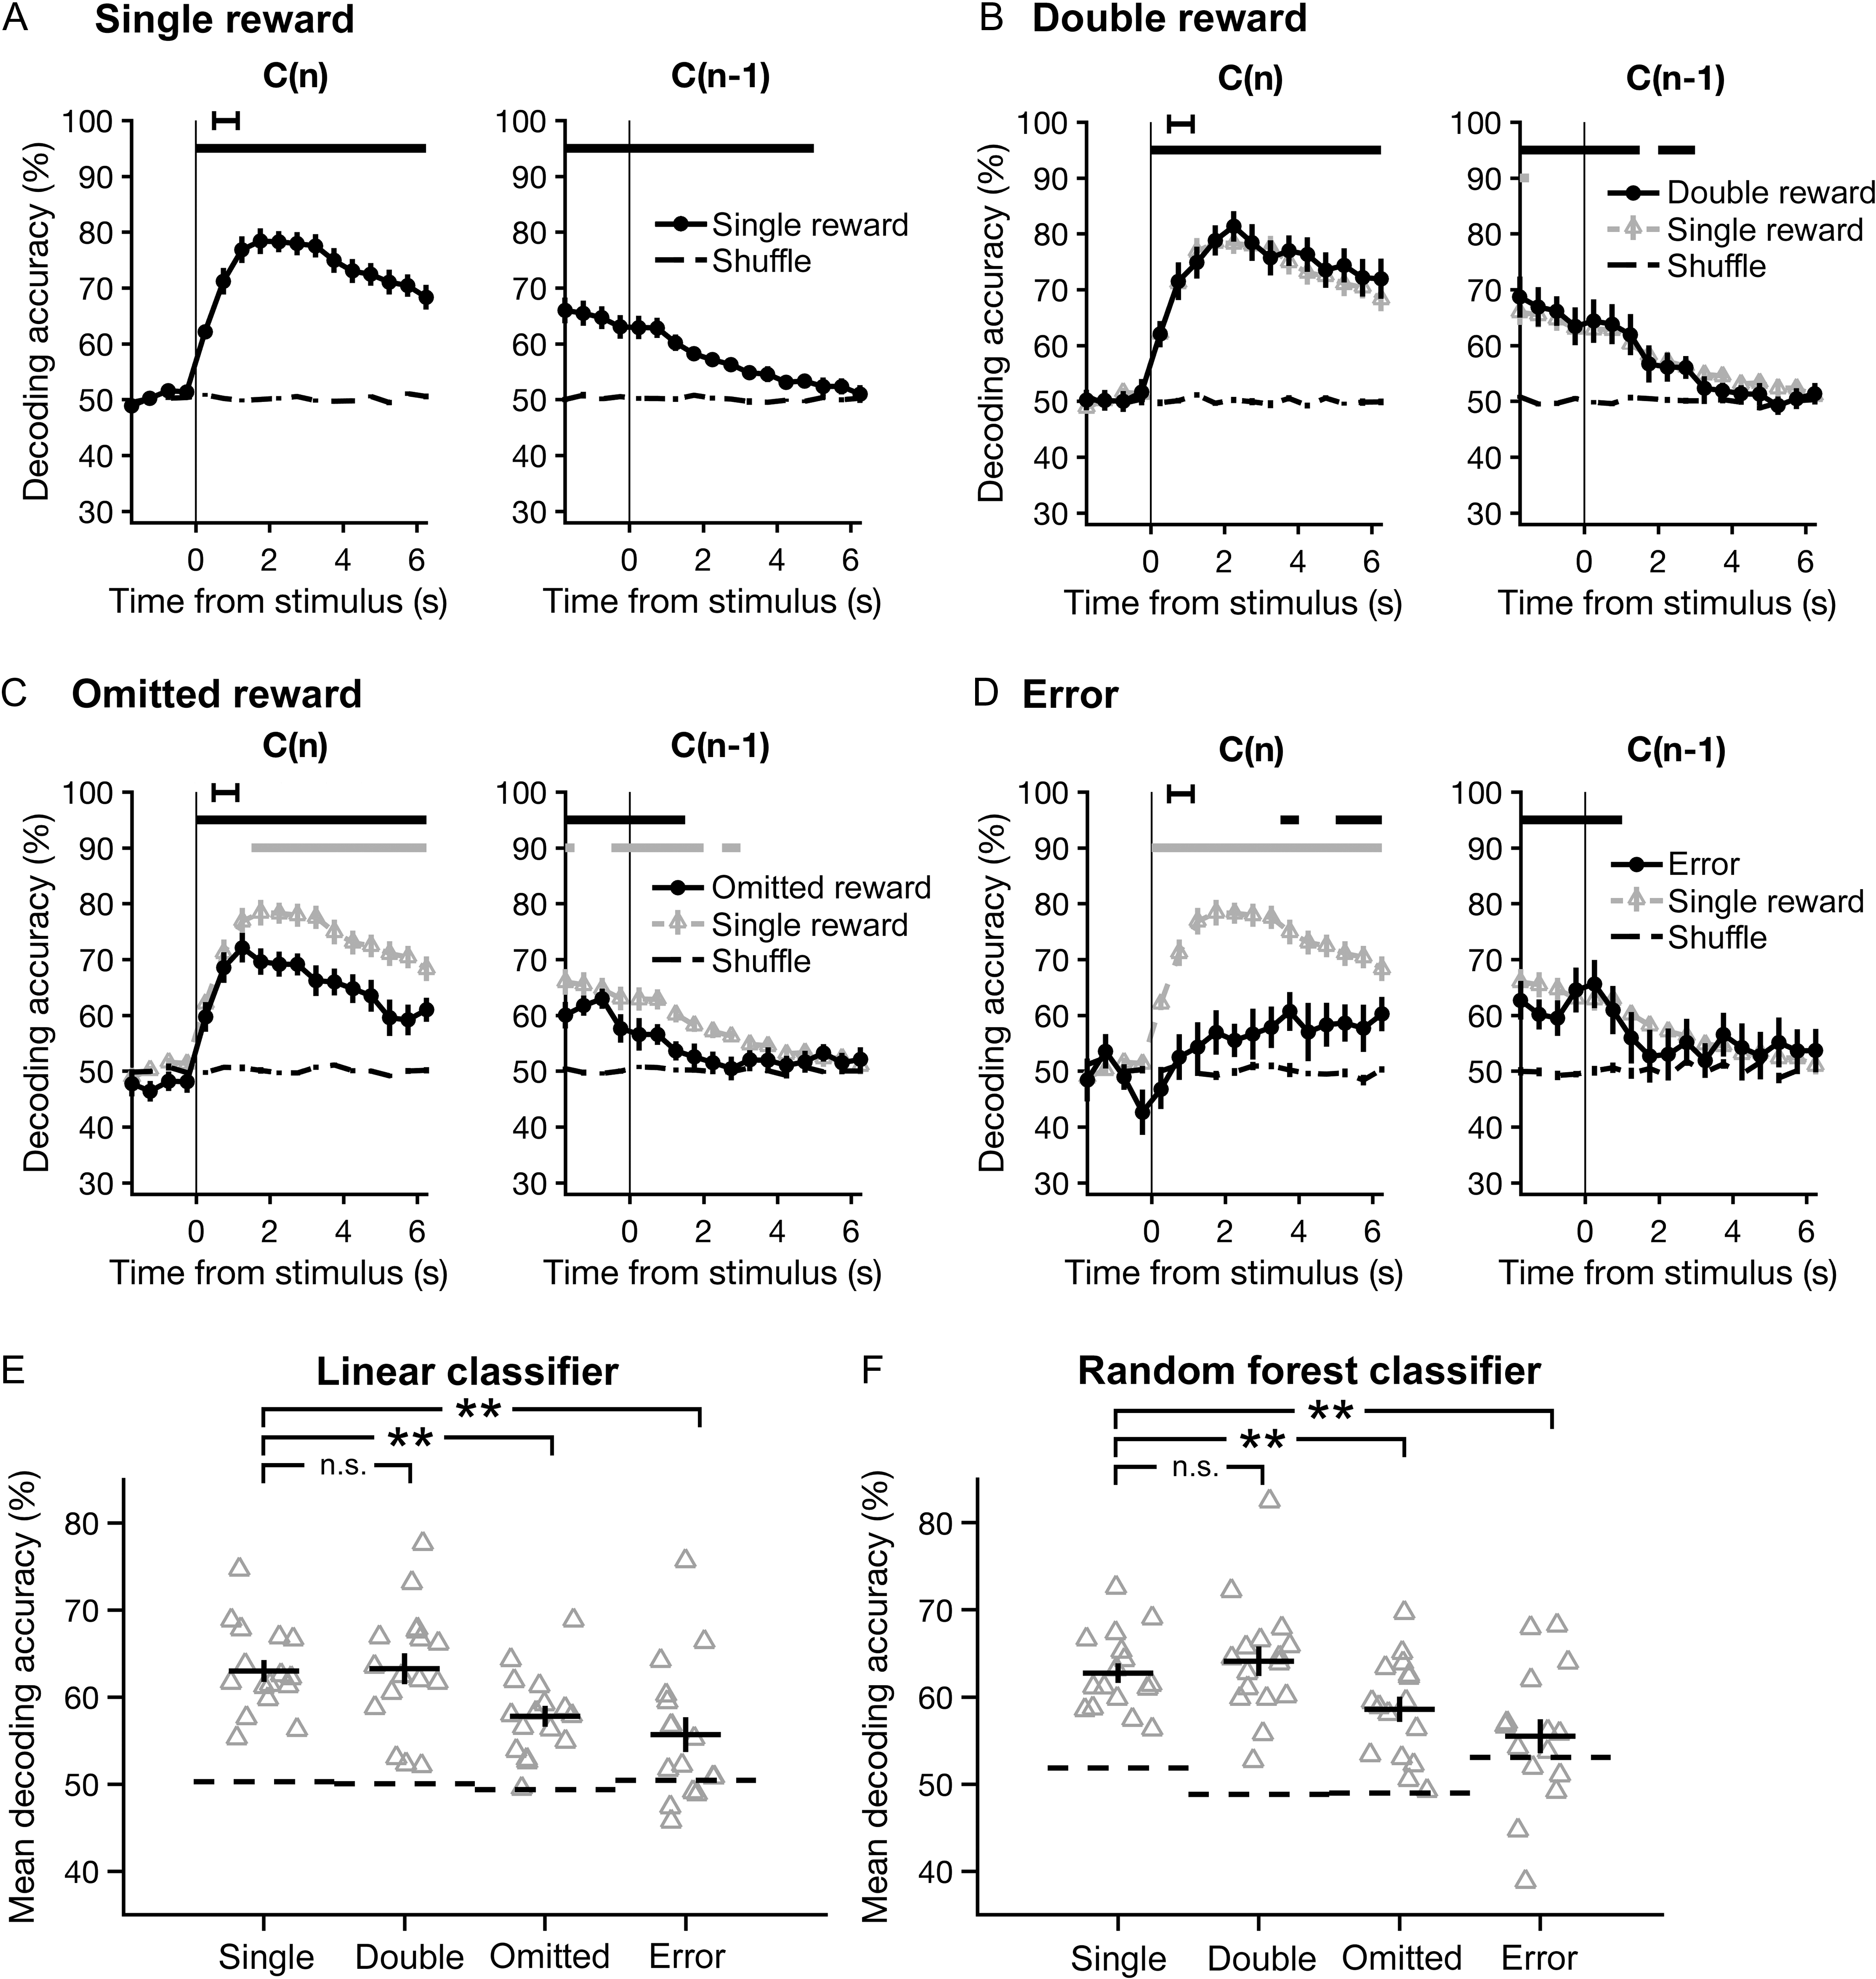
\includegraphics[width=\textwidth]{Figures/CC_fig6.png} 
% \end{center}
% \small{Figure \ref{fig:CC_fig6} Decoding accuracy diminished during omitted-reward and error trials. }